\documentclass{beamer}
%\usepackage{emoji}
\usepackage{fontawesome}
\usepackage{amsbsy}
\usepackage{amsmath}
\usepackage{amsthm}

\usepackage{pgfplots}
\usetikzlibrary{snakes,arrows,shapes}

\usepackage[mathscr]{euscript}
\usepackage{subcaption}
\usepackage{dblfloatfix}
\usepackage{fixltx2e}
\usepackage{color}
\usepackage{array, hhline}
\usepackage[normalem]{ulem}
\usepackage{rotating}
\usepackage{marvosym}
\usepackage{multirow}
\usepackage[mathscr]{euscript}
\usepackage{listings}
\usepackage{color}

\usetheme{Boadilla}
\title{My Presentation}
\subtitle{Using Beamer}
\author{Joe Bloggs}
\institute{University of ShareLaTeX}
\date{\today}


\newcommand{\vct}[1]{\ensuremath{\mathbf{#1}}}                                                    
\newcommand{\mtx}[1]{\ensuremath{\mathbf{\uppercase{#1}}}}                                   
\newcommand{\htr}[1]{\ensuremath{#1^\dagger}}
\newcommand{\dtm}[1]{\ensuremath{\lvert #1\rvert}}   
\newcommand{\im}{\ensuremath{i}}
\newcommand{\vhat}[1]{\ensuremath{\hat{\mathbf{#1}}}}

%\newcommand{\vre}{\ensuremath{v_{\vct{\xi}}}}

% Section, figure, table and equation references
\renewcommand{\eqref}[1]{(\ref{#1})}                                                    % equation reference
\newcommand{\Eqref}[1]{{Equation (\ref{#1})}}                                                      % Equation reference
\newcommand{\fgref}[1]{{Figure \ref{#1}}}                                                        % figure reference
\newcommand{\Fgref}[1]{{Figure \ref{#1}}}                                                        % Figure reference
\newcommand{\tbref}[1]{Table \ref{#1}}                                                               % table reference
\newcommand{\Tbref}[1]{Table \ref{#1}}                                                               % Table reference
\newcommand{\cpref}[1]{Chapter \ref{#1}}                                                             % chapter reference
\newcommand{\Cpref}[1]{Chapter \ref{#1}}                                                             % Chapter reference
\newcommand{\anref}[1]{{Appendix \ref{#1}}}                                                      % appendix reference
\newcommand{\Anref}[1]{{Appendix \ref{#1}}}                                                      % Appendix reference
\newcommand{\scref}[1]{{Section \ref{#1}}}                                                       % section reference
\newcommand{\Scref}[1]{{Section \ref{#1}}}                                                       % Section reference
\newcommand{\lmref}[1]{{Lemma \ref{#1}}}                                                       % lemma reference
\newcommand{\Lmref}[1]{{Lemma \ref{#1}}}                                                       % lemma reference

% Expected value
\newcommand{\expct}[1]{\ensuremath{\mathcal{E}\{#1\}}}                                          
\newcommand{\Expct}[1]{\ensuremath{\mathcal{E}\biggl\{#1\biggr\}}}  
\newcommand{\eex}[1]{\ensuremath{e^{#1}}}                                     
\newcommand{\ex}[1]{\ensuremath{\exp(#1)}}
\newcommand{\Ex}[1]{\ensuremath{\exp\biggl(#1\biggr)}}

\newcommand{\fdc}{\ensuremath{f_{\parm_{dc}}}}
\newcommand{\mtxIdentity}{\ensuremath{\mtx{I}}}

\newcommand{\pulse}{\ensuremath{z}}
\newcommand{\Pulse}{\ensuremath{Z}}
\newcommand{\envelope}{\ensuremath{p}}
\newcommand{\Envelope}{\ensuremath{P}}
\newcommand{\Snvelope}{\ensuremath{\mathscr{P}}}
\newcommand{\snvelope}{\ensuremath{\text{p}}}
\newcommand{\range}{\ensuremath{r}}
\newcommand{\rangeError}{\ensuremath{\delta_\range}}
\newcommand{\rangeErrorZero}{\ensuremath{\delta_{\range_0}}}
\newcommand{\stolt}{\ensuremath{\psi}}
\newcommand{\velocity}{\ensuremath{v}}
\newcommand{\acceleration}{\ensuremath{a}}
\newcommand{\sat}{\ensuremath{\vct{c}}}
\newcommand{\target}{\ensuremath{\vct{x}}}
\renewcommand{\d}{\ensuremath{\text{d}}}
\newcommand{\parm}{\ensuremath{s}}
\newcommand{\tparm}{\ensuremath{t}}
\newcommand{\fasttime}{\ensuremath{\tau}}
\newcommand{\satparm}{\ensuremath{\vct\sat(\parm)}}
\newcommand{\targetnoparm}{\ensuremath{\vct\target}}
\newcommand{\targetnoparmzero}{\ensuremath{\vct{x}_0}}
\newcommand{\uSatVelocity}[1]{\ensuremath{\vhat\velocity_\sat(#1)}}
\newcommand{\huSatVelocity}[1]{\ensuremath{\htr{\vhat\velocity}_\sat(#1)}}
\newcommand{\satVelocity}[1]{\ensuremath{\vct\velocity_\sat(#1)}}
\newcommand{\vtarget}{\ensuremath{\vct\velocity_\target}}
\newcommand{\hsatVelocity}[1]{\ensuremath{\htr{\vct\velocity}_\sat(#1)}}
\newcommand{\rcoeff}{\ensuremath{a}}

\newcommand{\targetVelocity}[1]{\ensuremath{\vct\velocity^\stationarySymbol_t(#1)}}
\newcommand{\rangeVectorParm}{\ensuremath{\vct{\range}(\parm, \targetnoparm)}}
\newcommand{\defrangeVectorParmZero}{\ensuremath{\vct{\range}(\parm_0, \targetnoparm_0)}}
\newcommand{\rangeVectorParmZero}{\ensuremath{\vct{\range}_0}}
\newcommand{\rangeVector}[1]{\ensuremath{\vct\range(#1)}}
\newcommand{\hrangeVector}[1]{\ensuremath{\htr{\vct\range}(#1)}}
\newcommand{\uRangeVectorParm}{\ensuremath{\vhat{\range}(\parm, \targetnoparm)}}
\newcommand{\defuRangeVectorParmZero}{\ensuremath{\vhat{\range}(\parm_0, \targetnoparm_0)}}
\newcommand{\uRangeVectorParmZero}{\ensuremath{\vhat{\range}_0}}
\newcommand{\uRangeVectorParmZeroPerp}{\ensuremath{\vhat{\range}_{0\bot}}}
\newcommand{\huRangeVectorParm}{\ensuremath{\htr{\vhat{\range}}(\parm)}}
\newcommand{\RangeVector}[1]{\ensuremath{\vct\range(#1)}}
\newcommand{\hRangeVector}[1]{\ensuremath{\htr{\vct\range}(#1)}}
\newcommand{\lat}{\ensuremath{\phi}_s}
\newcommand{\lng}{\ensuremath{\lambda}_s}
\newcommand{\rresolution}{\ensuremath{\delta_\range}}

\newcommand{\uRangeVector}[1]{\ensuremath{\vhat{\range}(#1)}}
\newcommand{\uRangeVectorl}[2]{\ensuremath{\vhat{\range}_{#1}(#2)}}
\newcommand{\huRangeVector}[1]{\ensuremath{\htr{\vhat{\range}}(#1)}}
\newcommand{\huRangeVectorl}[2]{\ensuremath{\htr{\vhat{\range}_{#1}}(#2)}}
\newcommand{\antennaPosition}[1]{\ensuremath{\vct{p}_{#1}}}
\newcommand{\pAntennaParm}[1]{\ensuremath{\vct{p}_{#1}(\parm)}}
\newcommand{\pAntennaParms}[1]{\ensuremath{\vct{p}_{#1}(\parm_s)}}
\newcommand{\pAntenna}[2]{\ensuremath{\vct{p}_{#1}(#2)}}
\newcommand{\xAntennaNoParm}[1]{\ensuremath{\vct{p}_{#1}}}
\newcommand{\xAntenna}[2]{\ensuremath{\xAntennaNoParm{#1}(#2)}}
\newcommand{\kr}{\ensuremath{k_r}}
\newcommand{\krn}{\ensuremath{k_{r'}}}
\newcommand{\krstolt}{\ensuremath{k_{r_s}}}
\newcommand{\krc}{\ensuremath{\krn}}
\newcommand{\krnaught}{\ensuremath{k_{r_0}}}
\renewcommand{\r}{\ensuremath{r_0}}
\newcommand{\xparm}{\ensuremath{\parm}}
\newcommand{\stationaryparm}{\ensuremath{\parm_p}}
\newcommand{\kparm}{\ensuremath{k_{\xparm}}}
\newcommand{\kparmPRF}{\ensuremath{k_{\xparm_p}}}
\newcommand{\gfunc}{\ensuremath{g}}
\newcommand{\myparm}{\ensuremath{\parm^*}}

% Signal in different domains
\newcommand{\ztzt}[1]{\ensuremath{zz_{#1}}}
\newcommand{\stst}[1]{\ensuremath{ss_{#1}}}
\newcommand{\Sfst}[1]{\ensuremath{Ss_{#1}}}
\newcommand{\SfSf}[1]{\ensuremath{SS_{#1}}}
\newcommand{\Skst}[1]{\ensuremath{\mathscr{S}s_{#1}}}
\newcommand{\SkSf}[1]{\ensuremath{\mathscr{S}S_{#1}}}
\newcommand{\SkSk}[1]{\ensuremath{\mathscr{S}\mathscr{S}_{#1}}}
\newcommand{\srSk}[1]{\ensuremath{s\mathscr{S}_{#1}}}
\newcommand{\SkSkM}{\ensuremath{\mtx{S}}}
\newcommand{\ststV}{\ensuremath{\boldsymbol{s}\boldsymbol{s}}}
\newcommand{\SfstV}{\ensuremath{\boldsymbol{S}\boldsymbol{s}}}
\newcommand{\SkstV}{\ensuremath{\boldsymbol{\mathscr{S}}\boldsymbol{s}}}
\newcommand{\SkSkV}{\ensuremath{\vct{s}}}
\newcommand{\SkSfV}{\ensuremath{\boldsymbol{\mathscr{S}}\boldsymbol{S}}}
\newcommand{\ZkZkM}{\ensuremath{\vct{z}}}
\newcommand{\SkSkR}{\ensuremath{\mathscr{S}\mathscr{S}_{R}}}
\newcommand{\ZkZkR}{\ensuremath{\mathscr{Z}\mathscr{Z}_{R}}}
\newcommand{\NkNkM}{\ensuremath{\vct{n}}}
\newcommand{\NkNkMP}{\ensuremath{\boldsymbol{\nu}}}

\newcommand{\fparm}{\ensuremath{f_\parm}}
\newcommand{\fparmPRF}{\ensuremath{f_{\parm_p}}}
\newcommand{\rangepos}{\ensuremath{\vct\range}_0}
\newcommand{\uRangepos}{\ensuremath{\vhat{\range}}_0}
\newcommand{\rangevel}{\ensuremath{{\vct{\velocity}}}_0}
\newcommand{\uRangevel}{\ensuremath{{\vhat{\velocity}}}_0}
\newcommand{\rangeacc}{\ensuremath{{\vct{\acceleration}}}_0}
\newcommand{\channelIndex}{\ensuremath{n}}
\newcommand{\beamIndex}{\ensuremath{m}}
\newcommand{\pattern}[1]{\ensuremath{\text{A}_{#1}}}
\newcommand{\dPattern}[1]{\ensuremath{\text{D}_{#1}}}
\newcommand{\dazPattern}[1]{\ensuremath{\text{D}_{\text{az}_{#1}}}}
\newcommand{\delPattern}[1]{\ensuremath{\text{D}_{\text{el}_{#1}}}}
\newcommand{\dconstelPattern}{\ensuremath{\text{D}_{\text{el}}}}
\newcommand{\edPattern}[1]{\ensuremath{\text{E}_{#1}}}
\newcommand{\elementPattern}[1]{\ensuremath{\text{E}_{#1}}}
\newcommand{\magVec}[1]{\ensuremath{\lvert#1\rvert}}
\newcommand{\amplitude}[1]{\ensuremath{\mathnormal{#1}}}
\newcommand{\Tx}[1]{\ensuremath{\vct\target\text{\footnotesize{x}}_{#1}}}
\newcommand{\Rx}[1]{\ensuremath{\vct\range\text{\footnotesize{x}}_{#1}}}
\newcommand{\costFunction}[1]{\ensuremath{J}_{#1}}
\newcommand{\eVec}[1]{\ensuremath{\vct{e}_{#1}}}
\newcommand{\heVec}[1]{\ensuremath{\htr{\vct{e}}_{#1}}}
\newcommand{\ebVec}[1]{\ensuremath{\vct{b}_{#1}}}
\newcommand{\hbVec}[1]{\ensuremath{\htr{\vct{b}}_{#1}}}
\newcommand{\cost}{\ensuremath{\varrho}}
\newcommand{\kvec}{\ensuremath{\vct{k}}}
\newcommand{\kveczero}{\ensuremath{\kr, \kparm}}
\newcommand{\kvecl}{\ensuremath{\kr, \kparm + l\kparmPRF}}
\newcommand{\kargs}{\ensuremath{\kr,\kparm}}
\newcommand{\hkvec}{\ensuremath{\htr{\vct{k}}}}
\newcommand{\effrelvel}{\ensuremath{\velocity_e}}
\newcommand{\vsat}{\ensuremath{\velocity_\sat}}
\newcommand{\transmitSet}[1]{\ensuremath{\mathcal{T}_{#1}}}
\newcommand{\arrayVector}{\ensuremath{\vct{e}}}
\newcommand{\transmitVector}[1]{\ensuremath{\vct{T}_{x_{#1}}}}
\newcommand{\htransmitVector}[1]{\ensuremath{\htr{\vct{T}}_{x_{#1}}}}
\newcommand{\receiveVector}[1]{\ensuremath{\vct{R}_{x_{#1}}}}
\newcommand{\hreceiveVector}[1]{\ensuremath{\htr{\vct{R}}_{x_{#1}}}}
\newcommand{\receiveSet}[1]{\ensuremath{\mathcal{R}_{#1}}}
\newcommand{\spacing}{\ensuremath{d}}
\newcommand{\nadAngle}{\ensuremath{\phi_0}}
\newcommand{\numberChannels}{\ensuremath{N_c}}
\newcommand{\channelM}{\ensuremath{M}}
\newcommand{\uX}[1]{\ensuremath{\vct{\hat{x}}(#1)}}
\newcommand{\uY}[1]{\ensuremath{\vct{\hat{y}}(#1)}}
\newcommand{\uZ}[1]{\ensuremath{\vct{\hat{z}}(#1)}}

\newcommand{\targetx}{\ensuremath{x}}
\newcommand{\targety}{\ensuremath{y}}
\newcommand{\targetz}{\ensuremath{z}}
\newcommand{\squint}{\ensuremath{\vartheta_s}}

\newcommand{\re}{\ensuremath{r_e}}
\newcommand{\rs}{\ensuremath{r_s}}
\newcommand{\rxz}{\ensuremath{r_{xz}}}
\newcommand{\rxy}{\ensuremath{r_{xy}}}
\newcommand{\rzy}{\ensuremath{r_z}}
\newcommand{\omegas}{\ensuremath{\omega_s}}
\newcommand{\satECEFangular}{\ensuremath{\boldsymbol\omega}_\sat}
\newcommand{\angular}{\ensuremath{\hat{\boldsymbol\omega}_\sat}}
\newcommand{\depression}{\ensuremath{\phi}}
\newcommand{\targetdepression}{\ensuremath{\depression}}
\newcommand{\targetomega}{\ensuremath{\omegas\parm_0}}
\newcommand{\targetrange}{\ensuremath{\range}}
\newcommand{\targetxparm}{\ensuremath{\xparm_{\target}}}
\newcommand{\targetrangez}{\ensuremath{\range_0}}
\newcommand{\targetxparmz}{\ensuremath{\xparm_{t_0}}}
\newcommand{\targetdepressionz}{\ensuremath{\depression_{0}}}
\newcommand{\omegat}{\ensuremath{\omega_t}}
\newcommand{\thetat}{\ensuremath{\theta_0}}
\newcommand{\thetas}{\ensuremath{\theta_s}}
\newcommand{\Thetas}{\ensuremath{\Theta_s}}
\newcommand{\phaser}{\ensuremath{\Psi_r}}
\newcommand{\alongtrack}{\ensuremath{{\alpha_\parallel}_n}}
\newcommand{\alongtrackparm}[1]{\ensuremath{{\alpha_\parallel}_{#1}}}
\newcommand{\acrosstrack}{\ensuremath{{\boldsymbol{\alpha}_\perp}_n}}

\newcommand{\antennaVector}{\ensuremath{\vct{a}}}
\newcommand{\antennaMatrix}{\ensuremath{\mtx{H}}}
\newcommand{\antennaPhaseMatrix}{\ensuremath{\mtx{P}}}
\newcommand{\diagAntennaMatrix}{\ensuremath{\mtx{D}}}
\newcommand{\hrwsFilterMatrix}{\ensuremath{\mtx{B}}}
\newcommand{\anTx}[1]{\ensuremath{\vct{T}_{x_{#1}}}}
\newcommand{\anRx}[1]{\ensuremath{\vct{R}_{x_{#1}}}}
\newcommand{\txDelay}[1]{\ensuremath{\delta_{T_{#1}}}}
\newcommand{\rxDelay}[1]{\ensuremath{\delta_{R_{#1}}}}
\newcommand{\txAmp}[1]{\ensuremath{\text{A}_{T_{#1}}}}
\newcommand{\rxAmp}[1]{\ensuremath{\text{A}_{R_{#1}}}}
\newcommand{\bline}{\ensuremath{\vct{b}}}
\newcommand{\uzero}{\ensuremath{\vct{u}_\channelIndex}}
\newcommand{\txn}{\ensuremath{n'}}
\newcommand{\txm}{\ensuremath{m'}}
\newcommand{\txN}{\ensuremath{N'}}
\newcommand{\txM}{\ensuremath{M'}}
\newcommand{\mnDelay}{\ensuremath{\delta_{\txm\txn}}}
\newcommand{\xang}{\ensuremath{x}}
\newcommand{\shelp}[3]{\ensuremath{\psi(\xang;#1,#2,#3)}}

\newcommand{\dthetas}{\ensuremath{\dot\theta_s}}
\newcommand{\gweight}[1]{\ensuremath{D_{#1}}}
\newcommand{\hgweight}[1]{\ensuremath{\averageAntenna^*_{#1}}}
\newcommand{\reflectivity}{\ensuremath{g}}
\newcommand{\vkern}{\ensuremath{\varPhi}}
\newcommand{\vkernvect}{\ensuremath{\boldsymbol{\vkern}}}
\newcommand{\alphaSymbol}{\ensuremath{\alpha}}
\newcommand{\betaSymbol}{\ensuremath{\beta}}
\newcommand{\gammaSymbol}{\ensuremath{\gamma}}
\newcommand{\alphaComponent}[1]{\ensuremath{\alphaSymbol_{#1}}}
\newcommand{\betaComponent}[1]{\ensuremath{\betaSymbol_{#1}}}
\newcommand{\gammaComponent}[1]{\ensuremath{\gammaSymbol_{#1}}}

\newcommand{\ct}{\ensuremath{\cos\omega_e t}}
\newcommand{\st}{\ensuremath{\sin\omega_e t}}
\newcommand{\del}{\ensuremath{\vec{\nabla}}}
\newcommand{\grad}{\ensuremath{\Delta}}
\newcommand{\Pf}{\ensuremath{\mtx{P}_\vct{f}}}
\newcommand{\uf}{\ensuremath{\hat{\vct{f}}}}
\newcommand{\df}{\ensuremath{\dot{\vct{f}}}}
\newcommand{\sats}{\ensuremath{\vct{c}_s}}
\newcommand{\satp}{\ensuremath{\vct{c}_p}}
\newcommand{\satt}{\ensuremath{\vct{c}_t}}
\newcommand{\dx}{\ensuremath{\dot{\satt}}}
\newcommand{\dw}{\ensuremath{\dot{\vct{w}}}}
\newcommand{\uw}{\ensuremath{\hat{\vct{w}}}}
\newcommand{\ddx}{\ensuremath{\ddot{\satt}}}
\newcommand{\udx}{\ensuremath{\hat{\dot{\satt}}}}
\newcommand{\dddx}{\ensuremath{\dddot{\satt}}}
\newcommand{\Px}{\ensuremath{\mtx{P}_{\satt}}}
\newcommand{\Pdx}{\ensuremath{\mtx{P}_{\dx(t)}}}
\newcommand{\Itwo}{\ensuremath{\mtx{I}_2}}
\newcommand{\Qtwo}{\ensuremath{\mtx{Q}_2}}
\newcommand{\prt}[2]{\ensuremath{\frac{\partial #1}{\partial #2}}}
\newcommand{\dtv}[2]{\ensuremath{\frac{\text{d}#1}{\text{d}#2}}}
\newcommand{\dtvtwo}[2]{\ensuremath{\frac{\text{d}^2#1}{\text{d}#2^2}}}
\newcommand{\dtvthree}[2]{\ensuremath{\frac{\text{d}^3#1}{\text{d}#2^3}}}
\newcommand{\prttwoa}[2]{\ensuremath{\frac{\partial^2#1}{\partial#2^2}}}
\newcommand{\prttwob}[3]{\ensuremath{\frac{\partial^2#1}{\partial#2\partial#3}}}

%\newcommand{\satparm}{\ensuremath{\vct{c}(s)}}
%\newcommand{\target}{\ensuremath{\vct{P}}}
\newcommand\Index[1]{#1}
\newcommand{\gls}[1]{#1}

\newcommand{\prf}{\ensuremath{f_p}}
\newcommand{\antennaLength}{\ensuremath{L}}
\newcommand{\antennaLengthDesired}{\ensuremath{L_0}}
\newcommand{\antennaLengthEffective}{\ensuremath{L_M}}
\newcommand{\wavelength}{\ensuremath{\lambda}}

% Input from SURE.tex
\newcommand{\threeDB}{\ensuremath{\Theta}}
\newcommand{\threeDBDesired}{\ensuremath{\Theta_{0}}}
\newcommand{\threeDBEffective}{\ensuremath{\Theta_{M}}}
\newcommand{\satv}{\ensuremath{v_s}}
\newcommand{\aziBW}{\ensuremath{B_a}}
\newcommand{\aziRes}{\ensuremath{\delta_x}}
\newcommand{\prfEffective}{\ensuremath{\prf}}
\newcommand{\prfreal}{\ensuremath{f_M}}
\newcommand{\resxDesired}{\ensuremath{\delta_0}}
\newcommand{\phaseSep}{\ensuremath{d}}
\newcommand{\lookdirection}{\ensuremath{\hat{u}}}
\newcommand{\vecsigTime}{\ensuremath{\vct{z}}}
\newcommand{\vecsigFreq}{\ensuremath{\vct{Z}}}
\newcommand{\vecsigFreqSampled}{\ensuremath{\vct{Z}_s}}
\newcommand{\htrvecsigFreqSampled}{\ensuremath{\htr{\vct{Z}}_s}}
\newcommand{\phaseCentreLocation}[1]{\ensuremath{\vct{p}_{#1}}}
\newcommand{\temporalbaseline}{\ensuremath{d_t}}
\newcommand{\spatialbaseline}{\ensuremath{d_s}}
\newcommand{\opt}{\rm opt}
\newcommand{\weight}[1]{\ensuremath{z_{#1}}}
\newcommand{\Nbands}{\ensuremath{N_{b}}}
\newcommand{\costweight}{\ensuremath{\varrho}}
\newcommand{\winweight}[1]{\ensuremath{\zeta_{#1}}}
\newcommand{\Winweight}{\ensuremath{\boldsymbol{\zeta}}}
\newcommand{\vopt}[1]{\ensuremath{\vct{v}^{\cg{\opt}}_{#1}}}
\newcommand{\Vopt}{\ensuremath{\mtx{V}_{\cg{\opt}}}}
\newcommand{\eigval}[1]{\ensuremath{\lambda_{#1}}}
\newcommand{\eigvec}[1]{\ensuremath{\vct{u}_{#1}}}
\newcommand{\alert}[1]{\textcolor{blue}{#1}}
\newcommand{\ish}[1]{\textcolor{blue}{#1}}
\newcommand{\cg}[1]{{#1}}
\newcommand{\cgs}[1]{\textcolor{red}{\sout{#1}}}
% \newcommand{\ishfix}[3]{{\textcolor{cyan}{#1}}{\tiny\textcolor{magenta}{#2}}{\scshape\small\textcolor{red}{#3}}}
\newcommand{\ishfix}[3]{#1}
\newcommand{\figref}[1]{\figurename~\ref{#1}}
\newtheorem{theorem}{Theorem}[section]
\newtheorem{corollary}{Corollary}[section]
\newtheorem{lemma}{Lemma}[section]
\newtheorem{question}{Question}[section]
\newtheorem{Definition}{Definition}[section]
\newcommand{\figD}{\ensuremath{\phaseSep=M\resxDesired=11\resxDesired}}
\newcommand{\figL}{\ensuremath{\antennaLengthEffective=2M\resxDesired=22\resxDesired}}
\newcommand{\figWL}{\ensuremath{\antennaLength=2M^2\resxDesired=242\resxDesired}}
\newcommand{\carrier}{\ensuremath{f_0}}


\begin{document}
\begin{frame}
\frametitle{Classic Stripmap SAR}
\begin{itemize}
\item SAR azimuth antenna length $\antennaLengthDesired$ and azimuth resolution $\resxDesired$ related by
\begin{equation}
 \antennaLengthDesired = 2\resxDesired.
\end{equation}
\item View $\resxDesired$ as a function of required beamwidth (for wavelength $\wavelength$),
\begin{equation}
 \threeDBDesired \approx \frac{\wavelength}{\antennaLengthDesired} = \frac{\wavelength}{2\resxDesired}.
\end{equation}
\item Required spatial sampling is $\resxDesired$ which means, for platform velocity $\satv$, we need a PRF of
\begin{equation}
 \prfEffective = \frac{\satv}{\resxDesired}.
\end{equation}
\item To minimize $\resxDesired$, minimize $\antennaLengthDesired$ which maximizes $\threeDBDesired$.
\end{itemize}
\end{frame}
%
\begin{frame}
\frametitle{Maximize azimuth beamwidth}
\begin{figure}[h!]
\begin{center}
 \resizebox{!}{0.4\textheight}{\input{increaseLookAngles.pdf_tex}}
 \caption{Spotlight mode to increase range of look angles.}
 \label{fg:fivechan}
 \end{center}
\end{figure}
\begin{itemize}
\item It's not the beamwidth but the fact that the target/scene is viewed from a wide range of azimuth angles. 
\item A wide beamwidth is one way to achieve this.
\item Spotlighting (mechanical or electronic) is another 
\end{itemize}
\end{frame}
%
\begin{frame}
\frametitle{Approach}
\begin{itemize}
\item Divide total beamwidth into $\myChannelM$ parts
\begin{equation}
 \threeDBEffective = \frac{\threeDBDesired}{\myChannelM}=\frac{\wavelength}{2\myChannelM\resxDesired}.
\end{equation}
\item Each part needs an antenna of length
\begin{equation}
 \antennaLengthEffective = 2\myChannelM\resxDesired,
\end{equation}
\item and a PRF of
\begin{equation}
 \prfEffective = \frac{2\satv}{\wavelength}\threeDBEffective = \frac{2\satv}{\antennaLengthEffective} = \frac{\satv}{\myChannelM\resxDesired},
 \label{eq:requiredPRF}
\end{equation}
\item Arrange a set of antennas of length $\antennaLengthEffective$ in the azimuth direction and change the beam direction from pulse to pulse
\end{itemize}
\end{frame}
%
\begin{frame}
\frametitle{Five channel example with ideal PRF}
\begin{figure}[h!]
\begin{center}
 \resizebox{!}{0.7\textheight}{\input{fivechan.pdf_tex}}
 \caption{Five channel example. Circles denote the phase-centre location while the angle denotes the direction of the Tx and Rx patterns.}
 \label{fg:fivechan}
 \end{center}
\end{figure}
\end{frame}
%
\begin{frame}
\frametitle{Azimuth antenna configuration}
\begin{itemize}
\item Arrange a set of subarrays in the along track direction as illustrated. 
\item Two-way phase-centre separation will be $\phaseSep=\myChannelM\resxDesired$
\item With each subarray of length $2\myChannelM\resxDesired$, the total array length is
\begin{equation}
 \antennaLength = \myChannelM\antennaLengthEffective = 2\myChannelM^2\resxDesired.
\end{equation}
\end{itemize}
\begin{figure}[h!]
\begin{center}
 \resizebox{0.4\columnwidth}{!}{\input{antennaLengths.pdf_tex}}
 \caption{Antenna Lengths to achieve desired resolution for an example 11 channel system for a desired resolution of $\resxDesired$.}
 \label{fg:antennaLenghts}
 \end{center}
\end{figure}
\end{frame}
%
\begin{frame}
\frametitle{Example antenna lengths}
\begin{table}[h!]
\begin{center}
\caption{System parameters for $\resxDesired=0.1 \text{m}$ and $\satv=7500 \text{m/s}$. The swath is the simply related to the time between pulses without consideration of pulse length and margins.}
\label{tb:Simulation}
 \begin{tabular}{r|c|c|c|c}\\\hline
  {\bf $\channelM$} & {\bf $\antennaLengthEffective$ m} & {\bf $\antennaLength$ m} & {\bf $\prfEffective$ Hz} & {\bf Swath (slant-range Km)}\\\hline 
1 & 0.20 & 0.20 & 75000 & 2.00\\\hline
3 & 0.60 & 1.80 & 25000 & 6.00\\\hline
5 & 1.00 & 5.00 & 15000 & 10.00\\\hline
7 & 1.40 & 9.80 & 10710 & 14.00\\\hline
9 & 1.80 & 16.20 & 8330 & 18.00\\\hline
{\bf 11} & {\bf 2.20} & {\bf 24.20} & {\bf 6810} & {\bf 22.00}\\\hline
13 & 2.60 & 33.80 & 5760 & 26.00\\\hline
15 & 3.00 & 45.00 & 5000 & 30.00\\\hline
 \end{tabular}
 \end{center}
\end{table}
\end{frame}
%
\begin{frame}
\frametitle{Signal processing}
\begin{figure}[h!]
\begin{center}
 \resizebox{0.9\textwidth}{!}{\input{equivalentHRWS.pdf_tex}}
 \caption{Equivalent HRWS system.}
 \label{fg:equivHRWS}
 \end{center}
\end{figure}
\begin{itemize}
\item Have to generalize to non-ideal PRFs.
\item Similar approach to non-uniform sampling for HRWS mode.
\item Number of samples grows as $1/\resxDesired^2$ in both azimuth and range.
\item Developed a wavenumber processing approach
\begin{itemize}
\item Based on paramterisation by arclength
\item Generalised Stolt interpolation
\end{itemize}
\end{itemize}
\end{frame}
%
\begin{frame}
\frametitle{Simulation}
\begin{table}[ht!]
\begin{center}
 \caption{Simulation parameters}
 \label{tb:simulation}
 \begin{tabular}{r|l|l|l|l|l|l|l}
  {} & {\bf $f_p$} & {\bf $\antennaLength$} & {\bf $\antennaLengthEffective$} & {\bf $M$} & {Swath} & {\bf $\carrier$} & {\bf $B$}\\
 {mode}      & {Hz}    & m    & m   &   & km   & GHz  & MHz\\\hline
 {\bf 40 cm} & 4500.00 & 20.0 & 4.0 & 5 & 16.5 & 9.65 & 374.74\\\hline
 {\bf 30 cm} & 5000.00 & 21.4 & 3.6 & 6 & 13.5 & 9.65 & 499.65\\\hline
 {\bf 25 cm} & 5142.86 & 24.4 & 3.5 & 7 & 12.7 & 9.65 & 599.58\\\hline
 {\bf 20 cm} & 6428.57 & 19.6 & 2.8 & 7 & 7.5  & 9.65 & 749.48\\\hline
 {\bf 12 cm} & 7500.00 & 24.0 & 2.4 & 10 & 4.5 & 9.65 & 1249.14\\\hline
 {\bf 10 cm} & 8181.82 & 24.2 & 2.2 & 11 & 3.0 & 9.65 & 1498.96\\\hline
 \end{tabular}
 \end{center}
\end{table}
\begin{itemize}
\item swath width has been computed in the slant-range.
\begin{equation}
 \text{Swath}(f_p; \tau_p) = \left(1/f_p - 2*\tau_p\right)*\frac{c}{2}\times 90\%
\end{equation}
\item $\tau_p$ is the pulse duration, selected as $\tau_p=50\times10^{-6}$ s. 
\item 10\% margin incorporated.
\end{itemize}
\end{frame}
%
\begin{frame}
\frametitle{Processed signal}
\begin{figure}[ht!]
\begin{center}
\begin{subfigure}{0.4\textwidth}
 \resizebox{\columnwidth}{!}{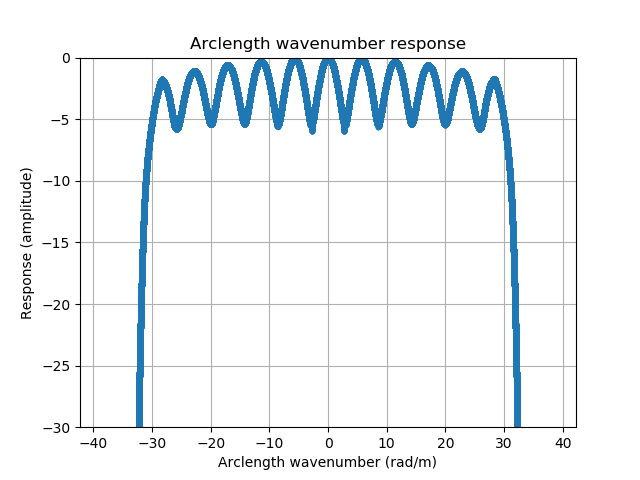
\includegraphics{simulation/10cm/simulation_plots_phase_corrected/wk_doppler_response_amplitude.png}}
 \caption{10 cm mode.}
 \label{fg:10cmreconstructed}
\end{subfigure}
\begin{subfigure}{0.4\textwidth}
 \resizebox{\columnwidth}{!}{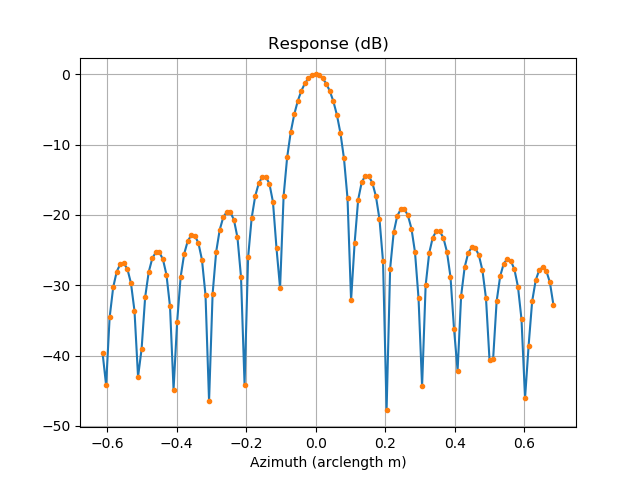
\includegraphics{simulation/10cm/simulation_plots_phase_corrected/wk_response_s_os_8.png}}
 \caption{Azimuth cross-section of 10cm mode.}
 \label{fg:azimuthCross10}
\end{subfigure}
\end{center}
\caption{Reconstructed signals in azimuth wavenumber domain.}
\label{fg:reconstructed}
\end{figure}
\end{frame}
%
\begin{frame}
\frametitle{PSF}
\begin{itemize}
\item Over the wider azimuth range, one observes a different generation of sidelobes with a peak rising to around -18dB. 
\item A Doppler weighting could suppress these at the expense of resolution.
\end{itemize}
\begin{figure}[ht!]
\begin{center}
 \resizebox{0.6\columnwidth}{!}{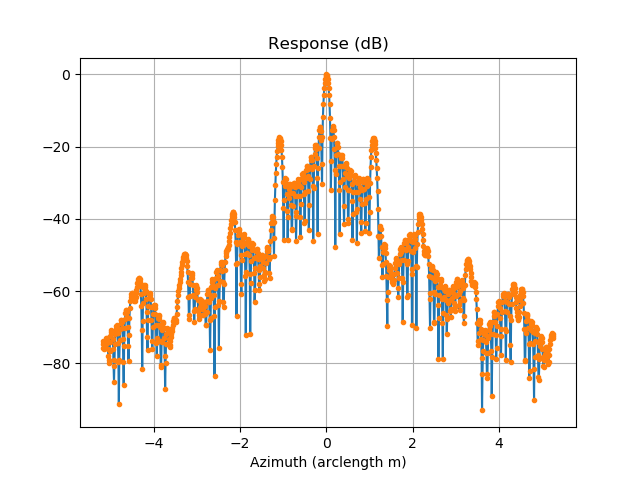
\includegraphics{simulation/10cm/simulation_plots_phase_corrected/wk_response_s_os_64.png}}
 \caption{Azimuth cross-section of 10cm mode.}
 \label{fg:azimuthCross10wide}
 \end{center}
\end{figure}
\end{frame}
%
\begin{frame}
\frametitle{NESZ}
\begin{table}[ht!]
\begin{center}
 \caption{Computed NESZ}
 \label{tb:nesz}
 \begin{tabular}{r|l|l}
 {\bf Mode} & {\bf $f_p$} (Hz)& {\bf NESZ} (dB)\\\hline
 {\bf 40 cm} & 4500.00 & -30.9\\\hline
 {\bf 30 cm} & 5000.00 & -29.8\\\hline
 {\bf 25 cm} & 5142.86 & -29.7\\\hline
 {\bf 20 cm} & 6428.57 & -29.2\\\hline
 {\bf 12 cm} & 7500.00 & -25.5\\\hline
 {\bf 10 cm} & 8181.82 & -30.2\\\hline
 \end{tabular}
 \end{center}
\end{table}
\end{frame}
\end{document}